\documentclass[11pt]{article}
\usepackage{mypackages}
\begin{document}

\subsection{Improving Policies}
\label{sec:improv}
Now that we can update and maintain an estimator of the value function, we want
to focus on improving the policy.
As for the value estimator, we learn the policy as a parameterized function $\pi(a, s, \theta_t)$
, which given an action $a$ and a state $s$ returns the probability
of taking action $a$ in state $s$ using the weights $\theta_t$.
The goal of the learning agent is to find the best policy, which is the one 
that will maximise the expected return.
To examine how well a policy is doing, we use a \textit{performance measure}, $\rho(\theta_t)$, to evaluate
the policy based on the policy weights $\theta_t$.
We want to maximise the performance measure since the policy is then optimal with
respect to $\rho(\theta_t)$.
As in section \ref{sec:td},
we perform gradient ascent to find the optimal weights of the performance measure,
and therefore, updating the policy weights is defined as
\begin{equation}
    \theta_{t+1} = \theta_t + \alpha \nabla_{\theta} \rho(\theta_t)
\end{equation}
where $0 < \alpha$ is a parameter determining the step size of the gradient ascent.

We want the performance measure to take all actions equally into account.
If an action has a high probability of being sampled, the weights are
updated more often with respect to that action, than for actions with a low probability of being sampled.
We make up for this imbalance by choosing a performance measure
that scales the gradient based on the probability of an action being sampled.
Such a performance measure can be constructed as
\begin{equation}
    \begin{aligned}
        \rho(\theta_t) & = \log\pi(a|s, \theta_t)
    \end{aligned}
\end{equation}
since taking the gradient would then result in
\begin{equation}\label{per_mes}
    \begin{aligned}
        \nabla_{\theta} \log\pi(a|s, \theta_t) = \frac{\nabla_{\theta}\pi(a|s, \theta_t)}{\pi(a|s,\theta)}
    \end{aligned}
\end{equation}
which means the probability of taking an action increases the magnitude of the gradient,
such that all actions should influence the weights the same over time.

Using this performance measure means we can't allow policies to become \textit{deterministic},
since having probability one for picking a single action would make the probabilities
of sampling the other actions zero, which means we would be dividing by zero
in equation \ref{per_mes}.

We can solve this problem by choosing our policy in a way that doesn't allow probabilities that are zero or one.
In this project, we will be using the \textit{softmax} function to achieve this,
by using a numerical preference $h(s, a, \theta) \in \mathbb{R}$
for each action available from the state $s$.
The numerical preference can be constructed in many ways, and we have chosen to use
a \textit{neural network} to estimate this preference for each action.
This means that the softmax function over the numerical preferences can be used to create a policy
as shown below. 
\begin{equation}\label{eq:soft_max}
    \pi(a | s, \theta_t) = \frac{e^{h(s,a,\theta_t)}}{\sum\limits_{a} e^{h(s,a,\theta_t)}}
\end{equation}

\subsubsection{The Actor-Critic Model}\label{sec:actor_critic}

A problem with the performance measure from equation \ref{per_mes} is that
the updates don't take rewards earned into account. 
To avoid updating without taking the rewards into account, we can
use the value function to evaluate the policy.
Combining the parameterized value function, $\hat{v}(s, \mathbf{w}_t)$,
and the parameterized policy, $\pi(a|s, \theta_t)$ is the basis of \textit{Actor-Critic} methods.
In the agent-environment model, the agent interacted with the environment
by performing actions and transitioning to new states.
For Actor-Critic methods, the agent-environment model is extended such that the agent,
or \textit{actor}, is still interacting with the environment, but
instead of only receiving the reward and new state, it also receives
a \textit{critique} of its performance - the TD-error.

\begin{figure}[!h]
    \centering
    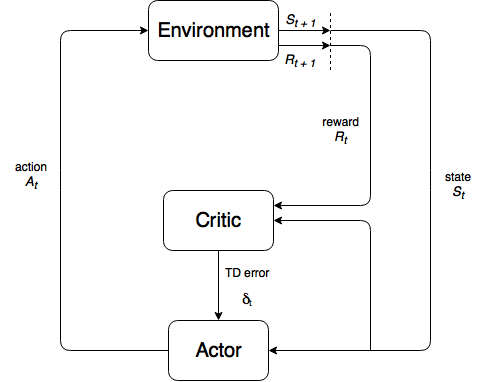
\includegraphics[scale = 0.5]{include/ActorCriticDiagram.png}
    \caption{A representation of the Actor-Critic Model.
        The environment sends a state and reward signal to both the actor and the critic.
        The critic computes the TD-error, which the actor uses as an evaluation of its performance
        and then picks a new action and so forth.}
    \label{fig:actor-critic}
\end{figure}
\newpage
This means that after an action sampled from $\pi(a|s,\theta_t)$ is performed,
the reward obtained for performing the action is used by the value estimator to
compute the one-step TD-error from section \ref{sec:td}.
\begin{equation*}
    \delta_t =  R_t + \gamma \hat{v} (S_{t+1}, \mathbf{w_t}) - \hat{v}(S_t, \mathbf{w_t})
\end{equation*}
The error is used to update the parameters of the policy,
as a way to weight the performance measure - if the TD-error is low,
the gradient step should be small, and vice versa.
\begin{equation}\label{eq:ac_theta}
    \theta_{t+1} = \theta_t + \delta_t \nabla_{\theta} \log \pi(A | S, \theta_t)
\end{equation}
This way of using the value function and policy is called an
\textit{Actor-Critic} method, where the policy can be seen as an actor
which is able to interact with the environment, while the value function
is the critic, evaluating the actions of the actor and 
influencing the policy accordingly.

%An advantage of using Actor-Critic methods is that the split into a actor and critic, reduces the variance of the function approximation, because the update step size for the policy parameters is defined relative to estimated value from critic.\cite{actCrit}

\subsubsection{Applying Eligibility Traces to the Actor-Critic Method}\label{sec:actor_critic_el}

To increase the stability of the Actor-Critic method, we can extend it to use eligibility traces
for the weights of the policy and value estimators.
As described in section \ref{sec:et}, eligibility traces can be seen as the weighted trend
of the most recent gradient updates, and they can be updated as
\begin{equation}
    \mathbf{e}^{\theta} = \lambda \mathbf{e}^{\theta} + \nabla_\theta \log\pi(a|s,\theta_t)
\end{equation}
and
\begin{equation}
    \mathbf{e}^{\mathbf{w}} = \lambda \mathbf{e}^{\mathbf{w}} + \nabla_\mathbf{w} \hat{v}(s, \mathbf{w}_t)
\end{equation}

This has a stabilising effect since it handles the problem of delayed reward.
For example in most Atari games performing an action doesn't immediately return a reward,
which means that the wrong actions might be reinforced due to the illusion
of those actions being responsible for the gained reward.
In section \ref{sec:et} the weight update of the value estimator
using an eligibility trace was presented as the trace weighted by
the one-step TD-error.
To gain more control of the gradient steps, the step-size parameters $\alpha$ and $\beta$ are used,
to avoid traversing too far in the direction of the gradient.
\begin{equation*}
    \mathbf{w}_{t+1}= \mathbf{w}_t + \alpha \delta \mathbf{e}^{\mathbf{w}}
\end{equation*}
Equivalently the weights of the policy estimator can be updated in the same fashion
\begin{equation}
    \theta_{t+1} = \theta_t + \beta \delta \mathbf{e}^\theta
\end{equation}

Now we have a way to solve a problem solely from experience.
The Actor-Critic Model, and Reinforcement Learning in general is well suited
to solve problems with domains that are difficult to describe since
they need no prior knowledge of the environment.
Extending the Actor-Critic Model to use eligibility traces 
increases the usability of the method since the model is 
influenced less by poor decisions, which is especially helpful
when the actor explores the effects of actions with a low probability.

%\printbibliography
%\bibliography{citations}
%\bibliographystyle{plain}
\end{document}
